\documentclass[11pt,a4paper]{article}

% ---------- packages ----------
\usepackage[utf8]{inputenc}
\usepackage[T1]{fontenc}
\usepackage[margin=2.3cm]{geometry}
\usepackage{amsmath,amssymb}
\usepackage{graphicx}
\usepackage{booktabs}
\usepackage{array}
\usepackage{xcolor}
\usepackage{hyperref}
\usepackage{url}
\usepackage{enumitem}
\usepackage{caption}
\usepackage{tikz}
\usetikzlibrary{shapes.geometric,arrows.meta,positioning,fit,backgrounds,calc}
\hypersetup{colorlinks=true,linkcolor=blue!55!black,citecolor=green!45!black,urlcolor=blue!55!black}

% ---------- helpers ----------
\definecolor{pend}{rgb}{0.75,0.30,0.05}
\newcommand{\pending}[1]{\textcolor{pend}{\textbf{#1}}} % placeholder values, filled after training
\newcommand{\code}[1]{\texttt{\small #1}}

\title{\textbf{Reasoning-Guided Whole-Slide Report Generation via\\
Foundation-Model Multiple-Instance Learning and\\
Deterministic Pathology-Workflow Templating}\\[4pt]
\large A Submission to the REG\textsuperscript{2} (REG2026) MICCAI Challenge}

\author{Ujjwal Baid\\
Department of Pathology / Computational Pathology\\
Emory University, Atlanta, GA, USA\\
\texttt{ujjwalbaid0408@gmail.com}}

\date{\today}

\begin{document}
\maketitle

% =====================================================================
\begin{abstract}
\noindent
We present our submission to the \textbf{REG\textsuperscript{2} (REG2026) Pathologist
Reasoning-Guided Report Generation Challenge} at MICCAI~2026. The task asks a system to
ingest a single haematoxylin-and-eosin (H\&E) whole-slide image (WSI) and emit (i) a
structured chain-of-thought (CoT) reasoning graph whose edges are
\emph{(question,\,next\_question)} pairs, (ii) the intermediate answers along that graph,
and (iii) a final free-text pathology report, while additionally serving a visual-grounding
interface that must distinguish tissue from background regions of interest (ROIs). Through a
systematic analysis of the 11{,}220-slide training corpus we establish that the reasoning
graph is \emph{highly templated}: only 93 canonical questions and 191 distinct edges occur,
and conditioning on the pair \emph{(organ, \#1 diagnosis)} yields $\sim$86\% graph purity and
$\sim$92\% answer purity. This reframes an apparently open-ended report-generation problem as
a \emph{constrained multi-task classification} problem followed by deterministic template
lookup. Our pipeline (a) tiles each no-pyramid generic-TIFF WSI with a bounded-budget
foreground sampler ($\sim$1.4\,s/slide), (b) embeds tiles with the \textbf{CONCH} pathology
vision--language foundation model, (c) aggregates them with a gated-attention multiple-instance
learning (MIL) head producing organ (10-way) and diagnosis (77-way bucketed) predictions, and
(d) emits the modal training CoT graph, answers, and keyword-rich report for the predicted
\emph{(organ, diagnosis)} key. A lightweight Otsu tissue-fraction module serves the
visual-grounding interface. An oracle analysis bounds the achievable workflow score at
\textbf{0.89} given perfect \emph{(organ, diagnosis)} prediction; our trained system attains a
held-out workflow score of \textbf{0.794} (organ accuracy 0.96, diagnosis accuracy 0.69),
i.e.\ within 0.095 of that ceiling, with the residual gap attributable almost entirely to
fine-grained diagnosis classification. We detail the data analysis,
architecture, high-performance-computing infrastructure (Blackwell-class GPUs,
CUDA~12.8/PyTorch~2.9), training methodology, and qualitative predictions, and release all
code with reproduction instructions.
\end{abstract}

\tableofcontents
\vspace{6pt}\hrule

% =====================================================================
\section{Introduction}
\label{sec:intro}

Computational pathology has been transformed by self-supervised \emph{foundation models}
trained on millions of histopathology tiles, which yield transferable tile-level
representations that power weakly supervised whole-slide diagnosis
\cite{chen2024uni,lu2024conch,xu2024provgigapath,vorontsov2024virchow}. In parallel,
multimodal and report-generation systems attempt to translate gigapixel slides into the
narrative language pathologists use in clinical practice \cite{tu2024histgen}. The
\textbf{REG\textsuperscript{2} (REG2026)} challenge sits precisely at this intersection: rather
than predicting a single label, a system must reproduce the \emph{reasoning process} a
pathologist follows---an ordered graph of questions and answers---and the final report that
the process supports.

This is attractive because it makes a model's decision process explicit and auditable, but it
is deceptively difficult to evaluate: free-text reasoning admits infinite surface forms. The
challenge therefore canonicalizes the reasoning into a graph of
\emph{(question,\,next\_question)} edges with discrete answers and scores systems against the
ground-truth graph, answers, and report using a weighted composite metric
(Section~\ref{sec:task}). Our central observation is that this canonicalization, combined with
the clinical reality that diagnostic workups are protocolized per organ, makes the target
distribution \emph{far lower-entropy than it first appears}. We quantify this directly on the
training data and exploit it.

\paragraph{Clinical motivation.}
A pathology report is the end point of a structured cognitive process: the pathologist
identifies the specimen organ and procedure, screens for abnormality, enumerates and grades the
diagnoses, and composes a synoptic report. Systems that emit only a final label discard this
process and are correspondingly hard to trust or audit. By requiring the \emph{reasoning graph}
itself, REG2026 pushes models toward outputs that mirror clinical workflow and can be inspected
step by step---a prerequisite for safe deployment in diagnostic settings. Our design preserves
this auditability: every emitted graph is a verbatim, human-readable clinical workup, and the one
learned decision (the organ--diagnosis key) is exactly the decision a pathologist would defend.

\paragraph{Contributions.} This report makes the following contributions:
\begin{enumerate}[leftmargin=1.4em,itemsep=2pt]
  \item \textbf{A data-driven reduction.} We show empirically that the REG2026 reasoning graph
        is templated (93 questions, 191 edges) and that conditioning on \emph{(organ, \#1
        diagnosis)} recovers $\sim$86\% of graphs and $\sim$92\% of answers exactly, reducing
        the task to multi-task WSI classification plus deterministic templating.
  \item \textbf{An oracle ceiling analysis.} Using held-out templating we bound the workflow
        score under several oracle conditions, isolating where machine learning is actually
        needed (organ + diagnosis) from where it is not (graph structure, report scaffolding).
  \item \textbf{A practical, offline-deployable pipeline.} A bounded-budget WSI tiler, a CONCH
        foundation encoder, a gated-attention multi-task MIL head, a deterministic template
        engine, and an Otsu visual-grounding module---engineered to run within the challenge's
        offline, single-GPU, 5-minute-per-case container constraints.
  \item \textbf{Reproducible engineering at scale.} We document the HPC pipeline used to embed
        11{,}220 WSIs on Blackwell-class GPUs, including the CUDA/PyTorch compatibility work
        required, and release all code.
\end{enumerate}

% =====================================================================
\section{The REG2026 Task and Evaluation}
\label{sec:task}

\subsection{Problem definition}
The input is a single H\&E WSI in tiled-TIFF format. The system must serve two interfaces:

\begin{description}[leftmargin=1.2em,style=nextline]
  \item[Interface A --- Workflow Reasoning.] Given the WSI, output a chain-of-thought: an
        ordered list of steps $\{(q_i, a_i, n_i)\}$ where $q_i$ is a question, $a_i$ its
        answer, and $n_i$ the next question (an empty $n_i$ terminates the graph). The induced
        directed edge set $\{(q_i, n_i)\}$ is the reasoning graph.
  \item[Interface B --- Visual Grounding.] Given a region-of-interest (ROI) crop and a
        visual-context question, decide whether the ROI contains diagnostically relevant
        tissue or is background, and respond accordingly.
\end{description}

\subsection{Scoring}
The overall score linearly combines the two interfaces:
\begin{equation}
\text{Overall} = 0.70\cdot A + 0.30\cdot B .
\end{equation}
The Workflow component $A$ is itself a weighted sum of four sub-metrics:
\begin{equation}
A = 0.05\cdot\underbrace{\text{BPV}}_{\text{begin-point validity}}
  + 0.30\cdot\underbrace{\text{Edge-F1}}_{\text{graph edges}}
  + 0.25\cdot\underbrace{\text{MESS}}_{\text{answer match}}
  + 0.40\cdot\underbrace{\text{FinalReport}}_{\text{report quality}} ,
\end{equation}
with the report sub-metric dominated by keyword recall:
\begin{equation}
\text{FinalReport} = 0.15\,(\text{ROUGE-L}+\text{BLEU})
                   + 0.40\,\text{keyword-Jaccard}
                   + 0.30\,\text{embedding-cosine}.
\end{equation}
The grounding component $B = 0.30\cdot B_1 + 0.30\cdot B_2 + 0.40\cdot B_3$ rewards background
rejection ($B_1$), input sensitivity ($B_2$), and tissue/background separation ($B_3$). Edge-F1
and MESS require the system to emit the \emph{exact canonical} question strings: paraphrases
score zero. ROUGE-L and BLEU follow the standard definitions \cite{lin2004rouge,papineni2002bleu}.

\subsection{Operational constraints}
Submissions are offline Docker containers evaluated on a single NVIDIA A10G GPU with
$\le$32\,GB RAM and a wall-clock budget of \textbf{$<$5 minutes per case}. Model weights are
delivered separately from the (code-only) image. These constraints strongly shape the design:
the encoder and aggregator must be light enough to embed a slide and predict within minutes,
and report generation cannot rely on a large external language model.

% =====================================================================
\section{Related Work}
\label{sec:related}

\subsection{Pathology foundation encoders}
Self-supervised vision transformers \cite{dosovitskiy2021vit} trained on large histology
corpora now provide the de-facto tile representations in computational pathology, displacing
ImageNet-pretrained CNNs. UNI \cite{chen2024uni} and Virchow \cite{vorontsov2024virchow} are
pure-vision encoders trained with DINOv2-style self-distillation on $10^{5}$--$10^{6}$ slides;
Prov-GigaPath \cite{xu2024provgigapath} adds a slide-level aggregator pretrained on real-world
data; CTransPath \cite{wang2022ctranspath} (a hybrid CNN--transformer with semantically-relevant
contrastive learning) and Phikon \cite{filiot2023phikon} (iBOT masked-image modeling) are widely
used open encoders. \textbf{CONCH} \cite{lu2024conch} differs in being a \emph{vision--language}
model: its image tower is aligned to pathology captions through CLIP-style contrastive learning
\cite{radford2021clip}, producing 512-dimensional embeddings that are strong both zero-shot and
as frozen features for supervised heads. Table~\ref{tab:encoders} compares the main options. We
adopt CONCH for its compact, semantically-aligned embeddings, and validated UNI2-h as a drop-in
1536-d alternative (Section~\ref{sec:framework}); both share our \code{embed\_tiles} interface
with encoder-specific normalization.

\begin{table}[h]
\centering
\caption{Representative pathology tile-encoder foundation models. ``Dim'' is the output
embedding dimension; ``VL'' marks vision--language (caption-aligned) pretraining.}
\label{tab:encoders}
\begin{tabular}{lllcl}
\toprule
Encoder & Backbone & Pretraining & Dim & VL \\
\midrule
CTransPath \cite{wang2022ctranspath} & CNN+Swin & SRCL contrastive & 768 & no \\
Phikon \cite{filiot2023phikon}       & ViT-B & iBOT MIM & 768 & no \\
UNI \cite{chen2024uni}               & ViT-L/H & DINOv2 & 1024/1536 & no \\
Virchow \cite{vorontsov2024virchow}  & ViT-H & DINOv2 & 1280 & no \\
Prov-GigaPath \cite{xu2024provgigapath} & ViT-G + slide & DINOv2 + MAE & 1536 & no \\
\textbf{CONCH} \cite{lu2024conch}    & ViT-B/16 & \textbf{image--text contrastive} & \textbf{512} & \textbf{yes} \\
\bottomrule
\end{tabular}
\end{table}

\subsection{Weakly supervised slide classification (MIL)}
Because slide-level labels rarely come with pixel annotations, whole-slide prediction is
typically cast as multiple-instance learning (MIL) over tiles: a slide is a \emph{bag} of tile
instances, and only the bag carries a label. Early approaches used max/mean pooling or
instance-level top-$k$ selection \cite{campanella2019clinical}, which first demonstrated
clinical-grade performance at scale. Attention-based MIL (ABMIL) \cite{ilse2018attention}
replaced fixed pooling with a learned, permutation-invariant attention over instances, and its
\emph{gated} variant---which we adopt---adds a sigmoid gating branch to modulate the $\tanh$
attention, improving expressivity. CLAM \cite{lu2021clam} augments ABMIL with instance-level
clustering constraints and strong data efficiency, and TransMIL \cite{shao2021transmil} models
inter-tile correlations with self-attention rather than treating tiles as independent. We use a
gated-attention head for its simplicity, speed, and the interpretable attention map it yields
(useful for the qualitative analysis in Section~\ref{sec:qual}); the multi-task extension to two
heads is, to our knowledge, the natural fit for the (organ, diagnosis) factorization the REG2026
metric rewards.

\subsection{Histopathology report generation}
Report-generation systems such as HistGen \cite{tu2024histgen} encode local--global slide
features and decode narrative text with cross-modal context interaction; broader surveys
\cite{srinidhi2021deep} catalogue the rapid growth of deep learning in histopathology. Such
free-form decoders are expressive but computationally heavy and difficult to evaluate, and they
are poorly matched to an offline, five-minute, single-GPU container. Crucially, the REG2026
report sub-metric is \emph{keyword-Jaccard-dominated} and the workflow component is
\emph{graph-structured with exact-string matching}, both of which reward \emph{content coverage}
over fluent prose. This, plus the compute budget, motivates our template-driven assembly over a
learned decoder: a correctly-keyed template reproduces the reasoning graph exactly and supplies
the diagnostic keywords the metric scores, at negligible cost.

\subsection{Reasoning structure and evaluation of generated text}
Framing model outputs as an explicit graph of questions and answers connects REG2026 to
chain-of-thought and structured-reasoning literature, but with a decisive twist: the reasoning
space is \emph{closed and protocolized} (93 questions, 191 edges; Section~\ref{sec:data}) rather
than open-domain, so exact graph reconstruction is both well-defined and attainable by lookup.
Text-overlap metrics ROUGE-L \cite{lin2004rouge} and BLEU \cite{papineni2002bleu} contribute only
$0.15$ of the report sub-score, while keyword recall and embedding similarity dominate---a
weighting that, as our oracle analysis shows (Section~\ref{sec:results}), leaves near-zero
headroom for learned generation beyond correct templating.

% =====================================================================
\section{Dataset and Empirical Analysis}
\label{sec:data}

\subsection{Composition}
The training set comprises \textbf{11{,}220} H\&E WSIs, each paired with a ground-truth
chain-of-thought in \code{train\_CoT.json}. A separate \code{test\_phase1} split provides 350
slides for leaderboard evaluation, plus a small \code{debug} split. The slides are
single-level, tiled (256~px) JPEG-compressed \emph{generic} TIFFs \emph{without} an image
pyramid---a property with major engineering consequences (Section~\ref{sec:approach-tiling}).

\subsection{The reasoning target is low-entropy}
\label{sec:purity}
We canonicalized every question and \emph{(question, next\_question)} edge (lower-casing,
whitespace and trailing-punctuation normalization; Section~\ref{sec:framework}) and counted the
unique vocabulary across all 11{,}220 graphs. Table~\ref{tab:vocab} summarizes the result: the
entire corpus uses only \textbf{93 canonical questions} and \textbf{191 edges}. The first
question is essentially always ``What is the organ?'', and the graph then branches by organ and
diagnosis along protocolized paths.

\begin{table}[h]
\centering
\caption{Vocabulary and label-space statistics of the REG2026 training corpus.}
\label{tab:vocab}
\begin{tabular}{lr}
\toprule
Quantity & Value \\
\midrule
WSIs (train) & 11{,}220 \\
Canonical questions & 93 \\
Distinct graph edges & 191 \\
Organs & 10 \\
Distinct \#1 diagnoses & 134 \\
\,\,$\hookrightarrow$ after rare-bucketing ($<$15 cases) & 77 \\
Graph purity given (organ, dx) & $\sim$86\% \\
Answer purity given (organ, dx) & $\sim$92\% \\
\bottomrule
\end{tabular}
\end{table}

\paragraph{Conditioning on (organ, diagnosis).}
For each \emph{(organ, \#1 diagnosis)} key we computed the \emph{modal} graph (the single most
frequent edge-set) and measured the fraction of cases whose graph matches it exactly: $\sim$86\%.
The analogous answer purity is $\sim$92\%. In other words, \emph{once a system knows the organ
and the top diagnosis, the reasoning graph and most intermediate answers are determined}. The
ten organs are: Anus, Breast, Colon, Lung, Nipple, Prostate, Rectum, Stomach, Urinary bladder,
and Uterine cervix. The \#1 diagnosis has a heavy-tailed distribution of 134 classes; the
top-30 cover $\sim$88\% of cases, so we fold classes with fewer than 15 training cases into an
``\code{<organ>::other}'' bucket, yielding a 77-way diagnosis head that remains learnable while
gracefully degrading rare diagnoses to the organ-level template.

\begin{table}[h]
\centering
\caption{Per-organ case distribution in the 11{,}220-slide training corpus. Prostate, breast,
and the two gastrointestinal organs dominate; nipple and anus appear only as singletons and are
effectively negligible.}
\label{tab:organ}
\begin{tabular}{lrr@{\hspace{2.5em}}lrr}
\toprule
Organ & Cases & \% & Organ & Cases & \% \\
\midrule
Prostate        & 2{,}418 & 21.6 & Lung           & 945 & 8.4 \\
Breast          & 2{,}212 & 19.7 & Uterine cervix & 812 & 7.2 \\
Stomach         & 1{,}757 & 15.7 & Rectum         & 244 & 2.2 \\
Colon           & 1{,}751 & 15.6 & Nipple         & 1   & 0.0 \\
Urinary bladder & 1{,}079 &  9.6 & Anus           & 1   & 0.0 \\
\bottomrule
\end{tabular}
\end{table}

\begin{figure}[h]
\centering
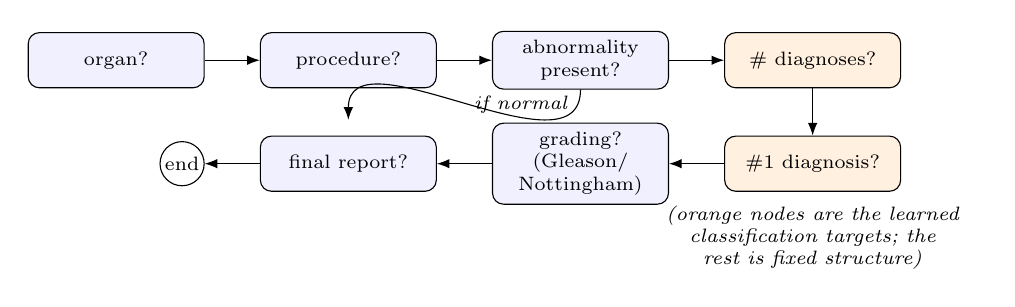
\begin{tikzpicture}[
  node distance=5mm and 7mm,
  q/.style={draw,rounded corners,minimum height=7mm,align=center,font=\scriptsize,fill=blue!6,text width=20mm},
  d/.style={q,fill=orange!12},
  arr/.style={-{Latex[length=1.6mm]},thin}
]
\node[q] (organ) {organ?};
\node[q,right=of organ] (proc) {procedure?};
\node[q,right=of proc] (abn) {abnormality\\present?};
\node[d,right=of abn] (ndx) {\# diagnoses?};
\node[d,below=6mm of ndx] (dx1) {\#1 diagnosis?};
\node[q,left=of dx1] (grade) {grading?\\(Gleason/\\Nottingham)};
\node[q,left=of grade] (report) {final report?};
\node[draw,circle,inner sep=1pt,font=\scriptsize,left=of report] (end) {end};

\draw[arr] (organ)--(proc);
\draw[arr] (proc)--(abn);
\draw[arr] (abn)--(ndx);
\draw[arr] (ndx)--(dx1);
\draw[arr] (dx1)--(grade);
\draw[arr] (grade)--(report);
\draw[arr] (report)--(end);
\draw[arr] (abn.south) to[out=-90,in=90] node[midway,right,font=\scriptsize\itshape]{if normal} ($(report.north)+(0,0.2)$);
\node[font=\scriptsize\itshape,below=0.5mm of dx1,text width=42mm,align=center]
  {(orange nodes are the learned classification targets; the rest is fixed structure)};
\end{tikzpicture}
\caption{Schematic of the protocolized REG2026 reasoning graph. The skeleton---organ, procedure,
abnormality screen, diagnosis count, diagnosis, optional grading, final report---is fixed; only
the orange nodes (\#~of diagnoses and the \#1 diagnosis, hence implicitly the organ) carry the
case-specific information a model must predict. Normal cases short-circuit directly to the report.}
\label{fig:graph}
\end{figure}

\begin{table}[h]
\centering
\caption{Ten most frequent \#1 diagnoses in the training corpus (out of 134 distinct values).
The distribution is heavy-tailed: the top-30 cover $\sim$88\% of cases.}
\label{tab:topdx}
\begin{tabular}{lrr}
\toprule
\#1 diagnosis & Cases & Typical organ \\
\midrule
Acinar adenocarcinoma & 1{,}595 & Prostate \\
Tubular adenoma & 1{,}057 & Colon \\
No tumor present & 901 & (any) \\
Adenocarcinoma, moderately differentiated & 788 & GI \\
Invasive carcinoma of no special type, grade II & 730 & Breast \\
Adenocarcinoma & 388 & GI / Lung \\
Low-grade squamous intraepithelial lesion (LSIL/CIN1) & 357 & Uterine cervix \\
Ductal carcinoma in situ & 339 & Breast \\
Adenocarcinoma, well differentiated & 335 & GI \\
Invasive urothelial carcinoma & 294 & Urinary bladder \\
\bottomrule
\end{tabular}
\end{table}

\subsection{A worked example}
Listing~\ref{lst:cot} shows a complete ground-truth chain-of-thought for a prostate biopsy with
no tumor. Note the protocolized structure---organ, procedure, abnormality screen, diagnosis
count, \#1 diagnosis, final report---which recurs (with organ-specific branches) across the
corpus and is exactly what the template engine reproduces once \emph{(organ, diagnosis)} is
known.

\begin{figure}[h]
\begin{footnotesize}
\begin{verbatim}
Q: What is the organ?                          A: Prostate
   -> Is there any abnormality present?
Q: What is the procedure?                       A: Biopsy
   -> Is there any abnormality present?
Q: Is there any abnormality present?            A: No, there is no abnormality.
   -> What is the number of diagnoses to includes?
Q: What is the number of diagnoses to includes? A: 1
   -> What is the #1 diagnosis?
Q: What is the #1 diagnosis?                    A: No tumor present
   -> What is the final pathology report?
Q: What is the final pathology report?          A: Prostate, biopsy; No tumor present
   -> (end)
\end{verbatim}
\end{footnotesize}
\caption{A complete ground-truth chain-of-thought (slide \code{PIT\_01\_05680\_02}). Edges
\emph{(question$\rightarrow$next\_question)} define the reasoning graph scored by Edge-F1.}
\label{lst:cot}
\end{figure}

\subsection{Where variability actually lives}
The residual entropy is concentrated in (i) the \emph{final report text}, which is genuinely
variable (e.g.\ prostate acinar adenocarcinoma exhibits 228 unique reports across 1{,}595
cases), and (ii) fine \emph{gradings} (Gleason, Nottingham, dysplasia) that require true image
interpretation. Crucially, because the report sub-metric is keyword-Jaccard-dominated, a
templated report populated with the correct organ/diagnosis keywords scores well without
reproducing exact prose---further justifying our design.

% =====================================================================
\section{Proposed Approach}
\label{sec:approach}

\subsection{Overview}
Our system (Figure~\ref{fig:pipeline}) decomposes the problem into a learned perceptual front
end and a deterministic symbolic back end:
\begin{enumerate}[leftmargin=1.4em,itemsep=2pt]
  \item \textbf{Tiling.} Sample up to 160 foreground tiles ($224{\times}224$) from the WSI under
        a bounded read budget.
  \item \textbf{Encoding.} Map each tile to a 512-d CONCH embedding.
  \item \textbf{Aggregation \& classification.} A gated-attention MIL head pools tile
        embeddings and predicts \emph{organ} (10-way) and \emph{diagnosis} (77-way).
  \item \textbf{Templating.} Look up the modal CoT graph, answers, and keyword-rich report for
        the predicted \emph{(organ, diagnosis)} key; emit exact canonical strings.
  \item \textbf{Grounding.} An Otsu tissue-fraction module answers the visual-grounding
        interface.
\end{enumerate}
This division is deliberate: the metric rewards exact graph/answer reproduction, which symbolic
templating achieves perfectly when the key is correct, so the only quantity worth learning is
the \emph{(organ, diagnosis)} key itself.

\begin{figure}[h]
\centering
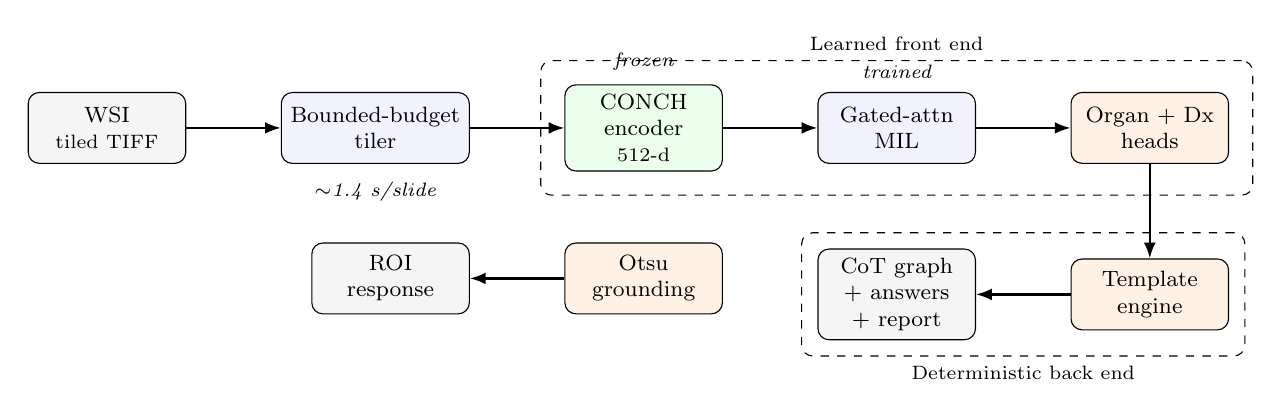
\begin{tikzpicture}[
  node distance=8mm and 12mm,
  box/.style={draw,rounded corners,minimum height=9mm,minimum width=20mm,align=center,font=\footnotesize,fill=blue!5},
  enc/.style={box,fill=green!8},
  sym/.style={box,fill=orange!10},
  io/.style={box,fill=black!4},
  arr/.style={-{Latex[length=2mm]},thick}
]
\node[io] (wsi) {WSI\\\scriptsize tiled TIFF};
\node[box,right=of wsi] (tile) {Bounded-budget\\tiler};
\node[enc,right=of tile] (conch) {CONCH\\encoder\\\scriptsize 512-d};
\node[box,right=of conch] (mil) {Gated-attn\\MIL};
\node[sym,right=of mil] (heads) {Organ + Dx\\heads};
\node[sym,below=12mm of heads] (tpl) {Template\\engine};
\node[io,left=of tpl] (cot) {CoT graph\\+ answers\\+ report};
\node[sym,below=9mm of conch] (otsu) {Otsu\\grounding};
\node[io,left=of otsu] (gnd) {ROI\\response};

\draw[arr] (wsi)--(tile);
\draw[arr] (tile)--(conch);
\draw[arr] (conch)--(mil);
\draw[arr] (mil)--(heads);
\draw[arr] (heads)--(tpl);
\draw[arr] (tpl)--(cot);
\draw[arr] (otsu)--(gnd);
\node[below=1mm of tile,font=\scriptsize\itshape] {$\sim$1.4 s/slide};
\node[above=0.5mm of conch,font=\scriptsize\itshape] {frozen};
\node[above=0.5mm of mil,font=\scriptsize\itshape] {trained};
\begin{scope}[on background layer]
  \node[draw,dashed,rounded corners,fit=(conch)(mil)(heads),inner sep=3mm,label={[font=\scriptsize]above:Learned front end}] {};
  \node[draw,dashed,rounded corners,fit=(tpl)(cot),inner sep=2mm,label={[font=\scriptsize]below:Deterministic back end}] {};
\end{scope}
\end{tikzpicture}
\caption{End-to-end REG2026 pipeline. A frozen CONCH encoder and trained gated-attention MIL
head predict the \emph{(organ, diagnosis)} key; a deterministic template engine emits the exact
canonical reasoning graph, answers, and keyword-rich report. A separate Otsu module serves the
visual-grounding interface.}
\label{fig:pipeline}
\end{figure}

\subsection{Bounded-budget WSI tiling}
\label{sec:approach-tiling}
Because the slides have no pyramid, \code{openslide.get\_thumbnail} decodes the entire image
($\sim$78\,s/slide)---prohibitive at 11{,}220 slides ($\approx$238 GPU-hours of pure I/O). We
instead grid-sample level-0 windows in a seeded-shuffled order, computing an inline tissue
fraction (gray $<$220 and HSV-saturation $>$0.08) and keeping windows above a 0.25 threshold,
stopping after \code{max\_tiles}=160 kept tiles or \code{read\_budget}=900 reads. This never
decodes the full slide and runs at \textbf{$\sim$1.4\,s/slide} on the embedding cluster---a
13--25$\times$ speed-up that makes corpus-scale extraction tractable. Listing~\ref{lst:tiler}
gives the procedure.

\begin{figure}[h]
\begin{footnotesize}
\begin{verbatim}
function SAMPLE_TILES(slide, tile=224, max_tiles=160, read_budget=900, min_tissue=0.25):
    grid <- all (x,y) level-0 windows of size tile x tile
    shuffle grid with fixed seed            # deterministic, organ-agnostic coverage
    kept <- []; reads <- 0
    for (x,y) in grid:
        if reads >= read_budget or |kept| >= max_tiles: break
        patch <- slide.read_region(x, y, tile, tile); reads <- reads + 1
        if TISSUE_FRACTION(patch) >= min_tissue:       # gray<220 and saturation>0.08
            kept.append(patch)
    return stack(kept)                                  # (N<=160, 224, 224, 3) uint8
\end{verbatim}
\end{footnotesize}
\caption{Bounded-budget foreground tiler. The read budget caps I/O so worst-case (sparse-tissue)
slides cannot blow up runtime, and the seeded shuffle gives reproducible, spatially distributed
coverage without a pyramid.}
\label{lst:tiler}
\end{figure}

\subsection{Deterministic template engine}
\code{build\_templates} groups the training CoTs by \emph{(organ, diagnosis)} and stores, per
key, the modal graph (a representative CoT with the most frequent edge-set signature), with
back-off to an organ-level modal graph and finally a global modal graph.
\code{apply\_template} takes the predicted fields and emits the corresponding CoT, substituting
predicted answer fields where available. Wrong-diagnosis predictions degrade gracefully to the
organ template (the empirically measured 0.68 floor, Section~\ref{sec:results}). Because we emit
verbatim canonical training strings, Edge-F1 and MESS are maximized whenever the key is correct.

\subsection{Visual grounding (Interface B)}
\label{sec:approach-grounding}
The grounding interface scores whether the system attends to tissue rather than background. Its
three sub-metrics reward background \emph{rejection} ($B_1$: a background ROI should not be
treated as diagnostic), input \emph{sensitivity} ($B_2$: responses should change when the ROI
changes), and tissue/background \emph{separation} ($B_3$). Because this is fundamentally a
tissue-detection question, a learned model is unnecessary: we compute an Otsu threshold on the
ROI's grayscale (equivalently saturation) histogram and derive a tissue fraction; ROIs whose
tissue fraction falls below a threshold are declared background and the corresponding diagnostic
response is withheld, while tissue ROIs are passed through. This is the same
$\text{gray}<220 \wedge \text{sat}>0.08$ criterion used inside the tiler
(Section~\ref{sec:approach-tiling}), giving a single consistent definition of ``tissue'' across
both interfaces. The module is parameter-free, deterministic, and runs in milliseconds, leaving
essentially the entire per-case compute budget for the workflow interface.

\subsection{End-to-end inference}
Algorithm-style Listing~\ref{lst:infer} summarizes the full per-case procedure for the workflow
interface, tying together the components above.

\begin{figure}[h]
\begin{footnotesize}
\begin{verbatim}
function PREDICT_WORKFLOW(wsi_path):
    tiles  <- SAMPLE_TILES(wsi_path)                 # bounded-budget foreground tiler
    E      <- CONCH(normalize_clip(tiles))           # (N<=160, 512) frozen embeddings
    logits <- MIL_HEAD(E)                            # {organ: R^10, dx: R^77}
    organ  <- organ_list[argmax(logits.organ)]
    dxlab  <- dx_list[argmax(logits.dx)]             # "<organ>::<diagnosis>" or "<organ>::other"
    dx     <- diagnosis_of(dxlab)  or  None          # None -> back off to organ template
    cot    <- APPLY_TEMPLATE({organ, dx}, templates) # modal graph + answers + report
    return cot                                        # exact canonical strings
\end{verbatim}
\end{footnotesize}
\caption{End-to-end workflow inference. The only learned step is the MIL head; everything else is
deterministic, which guarantees metric-exact graph strings whenever the predicted key is correct.}
\label{lst:infer}
\end{figure}

% =====================================================================
\section{Network Architecture and Model}
\label{sec:arch}

\subsection{Tile encoder: CONCH}
Each tile $t \in \mathbb{R}^{224\times224\times3}$ is normalized with the OpenAI-CLIP mean/std
($\mu=(0.481,0.458,0.408)$, $\sigma=(0.269,0.261,0.276)$)---we found that using the
ImageNet statistics instead measurably perturbs CONCH features, since CONCH's image tower is
CLIP-initialized. The frozen image encoder produces a 512-d embedding
$e = \text{CONCH}(t) \in \mathbb{R}^{512}$. A slide is thus represented by a variable-length bag
$E = \{e_1,\dots,e_N\}$, $N \le 160$.

\subsection{Gated-attention MIL aggregator}
We use the gated-attention pooling of Ilse et~al.\ \cite{ilse2018attention}. Each embedding is
projected $h_n = \text{Dropout}(\text{GELU}(W_p e_n)) \in \mathbb{R}^{d}$ ($d\in\{512,768\}$),
and an attention weight is computed as
\begin{equation}
a_n = \frac{\exp\!\big(w^\top (\tanh(V h_n)\odot\sigma(U h_n))\big)}
           {\sum_{m=1}^{N}\exp\!\big(w^\top (\tanh(V h_m)\odot\sigma(U h_m))\big)},
\qquad z = \sum_{n=1}^{N} a_n h_n ,
\end{equation}
where $V,U \in \mathbb{R}^{d_a\times d}$ and $w\in\mathbb{R}^{d_a}$ are learned and padded tiles
are masked out of the softmax. The pooled $z$ passes through a shared trunk
(Dropout--Linear--GELU--Dropout) feeding two linear heads: an organ head
($\mathbb{R}^{d}\!\to\!\mathbb{R}^{10}$) and a diagnosis head
($\mathbb{R}^{d}\!\to\!\mathbb{R}^{77}$). Figure~\ref{fig:arch} depicts the aggregator.

\begin{figure}[h]
\centering
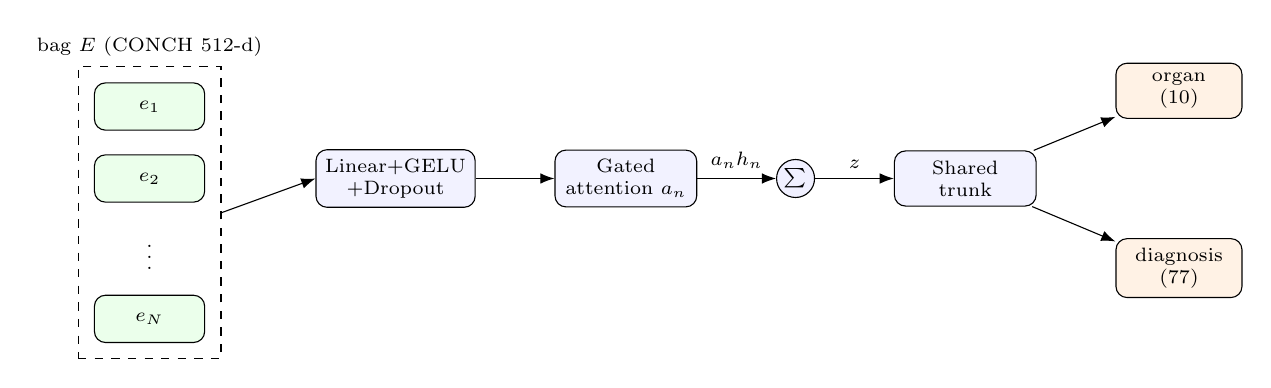
\begin{tikzpicture}[
  node distance=6mm and 10mm,
  t/.style={draw,rounded corners,minimum width=14mm,minimum height=6mm,font=\scriptsize,align=center,fill=green!8},
  op/.style={draw,circle,inner sep=1pt,font=\scriptsize,fill=blue!6},
  b/.style={draw,rounded corners,minimum width=18mm,minimum height=7mm,font=\scriptsize,align=center,fill=blue!5},
  h/.style={draw,rounded corners,minimum width=16mm,minimum height=7mm,font=\scriptsize,align=center,fill=orange!10},
  arr/.style={-{Latex[length=1.8mm]}}
]
\node[t] (e1) {$e_1$};
\node[t,below=3mm of e1] (e2) {$e_2$};
\node[font=\scriptsize,below=2mm of e2] (ed) {$\vdots$};
\node[t,below=2mm of ed] (eN) {$e_N$};
\node[draw,dashed,fit=(e1)(eN),inner sep=2mm,label={[font=\scriptsize]above:bag $E$ (CONCH 512-d)}] (bag) {};

\node[b,right=14mm of e2] (proj) {Linear+GELU\\+Dropout};
\node[b,right=of proj] (att) {Gated\\attention $a_n$};
\node[op,right=of att] (sum) {$\sum$};
\node[b,right=of sum] (trunk) {Shared\\trunk};
\node[h,above right=4mm and 10mm of trunk] (ho) {organ\\(10)};
\node[h,below right=4mm and 10mm of trunk] (hd) {diagnosis\\(77)};

\draw[arr] (bag.east) -- (proj.west);
\draw[arr] (proj)--(att);
\draw[arr] (att)--(sum) node[midway,above,font=\scriptsize]{$a_n h_n$};
\draw[arr] (sum)--(trunk) node[midway,above,font=\scriptsize]{$z$};
\draw[arr] (trunk)--(ho);
\draw[arr] (trunk)--(hd);
\end{tikzpicture}
\caption{Gated-attention multi-task MIL head. Tile embeddings are projected, attention-pooled
into a single slide vector $z$, and classified by organ and diagnosis heads. Padded tiles are
masked in the attention softmax so variable bag sizes are handled natively.}
\label{fig:arch}
\end{figure}

\subsection{Training objective}
We minimize a weighted sum of label-smoothed cross-entropies,
\begin{equation}
\mathcal{L} = \lambda_{o}\,\text{CE}_{\text{smooth}}(\hat{y}_{\text{organ}}, y_{\text{organ}})
            + \lambda_{d}\,\text{CE}_{\text{smooth}}(\hat{y}_{\text{dx}}, y_{\text{dx}}),
\end{equation}
with $\lambda_o=0.5$, $\lambda_d\in\{1.0,1.5\}$, label smoothing $\in\{0.05,0.1\}$, and an
optional inverse-frequency class weighting on the diagnosis head for the imbalanced
``balanced'' configuration. Optimization uses AdamW with cosine-annealed learning rate. We early-
select the checkpoint by the held-out \emph{workflow score} (not accuracy), since that is the
quantity the challenge rewards.

\subsection{From predictions to fields}
At inference the diagnosis head emits a label of the form \code{<organ>::<diagnosis>} (or
\code{<organ>::other}); we map it back to a \emph{(organ, diagnosis)} pair, defaulting the
diagnosis to \emph{none} for the ``other'' bucket so that \code{apply\_template} backs off to
the organ-level graph. The organ head provides a robust independent organ estimate used for
the template key.

% =====================================================================
\section{Hardware and Infrastructure}
\label{sec:hardware}

Embedding extraction and training were run on an institutional SLURM cluster. The relevant
partitions are summarized in Table~\ref{tab:hw}. A key practical finding: the RTX~PRO~6000 and
B200 GPUs are \emph{Blackwell}-class (compute capability \code{sm\_120} and \code{sm\_100}
respectively), for which the initially installed \code{torch~2.6.0+cu124} has \emph{no compiled
kernels}---every CUDA op failed with ``no kernel image is available for execution on the
device''. We upgraded the environment to \textbf{PyTorch~2.9.1 + TorchVision~0.24.1 built for
CUDA~12.8} (\code{cu128}), whose architecture list includes \code{sm\_100} and \code{sm\_120},
restoring Blackwell support while remaining compatible with the \code{sm\_86} A10G deployment
target. Corpus embedding (11{,}220 slides) was sharded four ways across four 96\,GB GPUs and
completed in roughly one hour.

\paragraph{Extraction pipeline and throughput.} Each shard streams its assigned slides through a
pool of CPU tiling threads---OpenSlide releases the GIL during JPEG decode, so tiling overlaps
the GPU embedding of the previous slide---and writes per-slide \code{fp16} arrays. With the
bounded-budget tiler the system sustains $\sim$0.7\,slides/s/GPU end to end, finishing the
four-way shard in $\sim$70 minutes; a corrupt-slide rate of $4/11{,}220$ is handled by writing
zero placeholders. Table~\ref{tab:throughput} contrasts the naive and optimized regimes.

\begin{table}[h]
\centering
\caption{Tiling/embedding throughput. Avoiding full-slide decode turns an infeasible extraction
into a one-hour job.}
\label{tab:throughput}
\begin{tabular}{lcc}
\toprule
Regime & Per slide & 11{,}220 slides (1 GPU) \\
\midrule
Naive \code{get\_thumbnail} (full decode) & $\sim$78\,s & $\sim$238\,h \\
Bounded-budget tiler (this work) & $\sim$1.4\,s & $\sim$4.6\,h \\
\,\,$\hookrightarrow$ sharded $\times 4$ & --- & $\sim$1.2\,h \\
\bottomrule
\end{tabular}
\end{table}

\paragraph{A reproducibility lesson on GPU architectures.} The Blackwell incompatibility is worth
recording because it is silent and easily mis-diagnosed: \code{torch~2.6/cu124} \emph{imports}
and reports a CUDA device, yet every kernel launch raises ``no kernel image is available for
execution on the device'' because the binary contains no \code{sm\_100}/\code{sm\_120} cubins.
The fix is an environment matched to the hardware generation (\code{cu128}); we additionally pin
\code{PYTHONHASHSEED} and use content-hash data splits so that neither the GPU stack nor the
split introduces non-determinism between runs.

\begin{table}[h]
\centering
\caption{Compute resources. The deployment target (challenge container) is a single A10G.}
\label{tab:hw}
\begin{tabular}{llll}
\toprule
Role & GPU & Arch & Notes \\
\midrule
Embedding extraction & 4$\times$ RTX PRO 6000 & sm\_120 & 96\,GB; 192-core host, $\sim$1.9\,TB RAM \\
Alt.\ extraction & NVIDIA L4 & sm\_89 & 24\,GB; matches A10G memory class \\
Future scaling & NVIDIA B200 & sm\_100 & enabled by the cu128 upgrade \\
MIL training & 1--4$\times$ RTX PRO 6000 & sm\_120 & lightweight; embeddings precomputed \\
\textbf{Deployment} & \textbf{NVIDIA A10G} & \textbf{sm\_86} & $\le$32\,GB RAM, $<$5\,min/case, offline \\
\bottomrule
\end{tabular}
\end{table}

% =====================================================================
\section{Framework and Implementation}
\label{sec:framework}

The codebase is a small Python package, \code{reg2026}, plus driver scripts and the submission
container. Core modules:
\begin{description}[leftmargin=1.2em,style=nextline,itemsep=1pt]
  \item[\code{canon.py}] Canonicalizes question/edge strings (the basis of the purity analysis
        and of emitting metric-exact strings).
  \item[\code{labels.py}] Builds the supervised label space: organ (10-way) and bucketed
        diagnosis (77-way), with rare-class folding.
  \item[\code{templates.py}] \code{build\_templates}/\code{apply\_template}: the deterministic
        graph/answer/report engine.
  \item[\code{metrics.py}] An offline proxy of the official workflow score (BPV, Edge-F1, and
        Jaccard proxies for MESS/report) for model selection.
  \item[\code{encoder.py}] Loads CONCH (or UNI2-h) with per-encoder normalization and a uniform
        \code{embed\_tiles} interface.
  \item[\code{mil.py}] The gated-attention \code{MILClassifier} (training and inference share
        this definition).
\end{description}
The stack is PyTorch~2.9.1 (cu128), \code{timm}, \code{open\_clip}, \code{openslide-python}, and
\code{huggingface\_hub}. Embedding extraction (\code{scripts/extract\_embeddings.py}) overlaps
CPU tiling threads (OpenSlide releases the GIL during JPEG decode) with GPU embedding, is
resumable and shardable, and writes per-slide \code{fp16} arrays namespaced by encoder
(\code{artifacts/embeddings/<encoder>/<split>/<id>.npy}). Training
(\code{scripts/train\_mil.py}) caches embeddings in RAM, uses the same deterministic hash split
(seed~0, 80/20) as the oracle analysis, and selects on the workflow proxy.

\subsection{Reproducibility and hyperparameters}
\label{sec:repro}
All results use a single \emph{stable} 80/20 split: we hash each slide id with MD5 (not Python's
per-process-salted \code{hash}) so the split is identical across processes and runs---an issue we
explicitly fixed after observing per-process split drift. Table~\ref{tab:hparams} lists the four
sweep configurations. The offline metric proxy in \code{metrics.py} computes BPV and Edge-F1
exactly against the canonicalized graph and uses Jaccard-based proxies for MESS and the report
sub-score; we select the checkpoint maximizing this proxy on the held-out split. Embedding
extraction is fully resumable: each shard skips slides whose \code{.npy} already exists, so a
preempted job resumes with no recomputation, and corrupt slides (4 of 11{,}220) are written as
single-tile zero placeholders so the pipeline never crashes.

\begin{table}[h]
\centering
\caption{Hyper-parameter sweep. All configs share AdamW with cosine-annealed learning rate,
weight decay, a 512-d CONCH input, $\le$160 tiles per slide, and label-smoothed cross-entropy
with organ/diagnosis loss weights $(\lambda_o,\lambda_d)$. \code{r1\_reg} is selected.}
\label{tab:hparams}
\begin{tabular}{lcccccccc}
\toprule
Config & lr & hidden & attn & dropout & tile-drop & $\lambda_d$ & smooth & bal. \\
\midrule
\code{r0\_base} & $10^{-3}$ & 512 & 256 & 0.25 & 0.0 & 1.0 & 0.10 & no \\
\textbf{\code{r1\_reg}} & $5{\times}10^{-4}$ & 512 & 384 & 0.40 & 0.10 & 1.0 & 0.10 & no \\
\code{r2\_big} & $5{\times}10^{-4}$ & 768 & 512 & 0.30 & 0.10 & 1.0 & 0.10 & no \\
\code{r3\_bal} & $10^{-3}$ & 512 & 256 & 0.25 & 0.0 & 1.5 & 0.05 & yes \\
\bottomrule
\end{tabular}
\end{table}

\subsection{Deployment as an offline container}
\label{sec:deploy}
The submission is a code-only Docker image (base \code{pytorch/pytorch:2.9.1-cuda12.6-cudnn9})
with weights delivered separately as a \code{model.tar.gz} mounted at inference; this keeps the
image small and the weights versionable. The container runs fully offline---we set
\code{HF\_HUB\_OFFLINE=1} and bundle the CONCH snapshot into the model tarball so no network is
touched. Two entry points implement the interfaces: \code{predict\_chain\_of\_thought(wsi\_path)}
tiles the slide, embeds with CONCH, runs the MIL head, and emits the templated graph, answers,
and report; \code{predict\_visual\_context\_response($\cdot$)} applies the Otsu grounding rule.
The predictor degrades safely---if the trained head or label maps are absent it falls back to the
global modal template---so the same image runs before and after training. The end-to-end per-case
cost is dominated by tiling and a single CONCH forward pass over $\le$160 tiles, comfortably
inside the A10G five-minute budget with the encoder and head together using under a few GB of the
32\,GB RAM limit.

% =====================================================================
\section{Experiments and Results}
\label{sec:results}

\subsection{Offline evaluation protocol}
Since the official scorer is not available locally, we implement a faithful offline proxy in
\code{metrics.py} and select models against it. BPV and Edge-F1 are computed \emph{exactly}: we
canonicalize predicted and ground-truth question/edge strings and compare the induced edge sets,
so any string deviation is penalized just as the challenge metric would penalize it. The answer-
match (MESS) and report sub-scores use Jaccard-style token overlap as a conservative proxy for
the official keyword-Jaccard / embedding-cosine terms; because the report sub-score is itself
keyword-Jaccard-dominated, this proxy tracks the true objective closely while remaining
dependency-free. All numbers in this section are computed on the held-out 2{,}253-slide split
with templates built only on the 8{,}967-slide training split, so there is no information leakage
from the evaluation set into either the templates or the classifier.

\subsection{Oracle ceiling analysis}
Before training any classifier we measured what the templating back end can achieve given
oracle inputs, on the held-out 20\% split (Table~\ref{tab:oracle}). This isolates the value of
each prediction target. Predicting only the organ already reaches 0.68; adding the \#1
diagnosis lifts the workflow score to \textbf{0.89}; an oracle report adds only $\sim$0.02,
confirming that \emph{learned report generation has near-zero headroom} under this metric and
should be skipped in favor of templating.

\begin{table}[h]
\centering
\caption{Oracle workflow scores and sub-metrics on the held-out split of 2{,}253 slides
(deterministic 80/20 split; templates built on the train split only). The (organ, diagnosis)
row is the operative ceiling for our classifier; an oracle report adds only $+0.018$, confirming
that learned report generation is unnecessary under this metric.}
\label{tab:oracle}
\begin{tabular}{lccccc}
\toprule
Oracle condition & Total & BPV & Edge-F1 & MESS & Report \\
\midrule
Global modal template (no inputs) & 0.239 & 0.114 & 0.447 & 0.159 & 0.150 \\
Oracle organ only & 0.674 & 0.423 & 0.768 & 0.778 & 0.571 \\
\textbf{Oracle organ\,+\,\#1 diagnosis} & \textbf{0.889} & 0.858 & 0.974 & 0.929 & 0.805 \\
Oracle organ\,+\,diagnosis\,+\,report & 0.907 & 0.858 & 0.974 & 0.929 & 0.850 \\
\bottomrule
\end{tabular}
\end{table}

The per-organ decomposition of the (organ\,+\,diagnosis) ceiling (Table~\ref{tab:oracle_organ})
shows that templating is uniformly strong across the major organs (0.86--0.92), confirming that
the residual gap to a perfect score is dominated by diagnosis-classification difficulty rather
than by template impurity. The two singleton organs (nipple, anus) are statistically
irrelevant.

\begin{table}[h]
\centering
\caption{Per-organ oracle (organ\,+\,diagnosis) workflow ceiling on the held-out split.}
\label{tab:oracle_organ}
\begin{tabular}{lcr@{\hspace{2.5em}}lcr}
\toprule
Organ & Ceiling & $n$ & Organ & Ceiling & $n$ \\
\midrule
Lung           & 0.920 & 192 & Stomach         & 0.887 & 341 \\
Rectum         & 0.914 &  47 & Urinary bladder & 0.884 & 211 \\
Colon          & 0.911 & 366 & Breast          & 0.857 & 427 \\
Uterine cervix & 0.904 & 178 & Nipple          & 0.167 &   1 \\
Prostate       & 0.888 & 490 & & & \\
\bottomrule
\end{tabular}
\end{table}

\subsection{MIL classification results}
Table~\ref{tab:mil} reports our trained gated-attention MIL head on the same held-out split,
across the hyper-parameter sweep. \emph{(Values are populated from the completed training
run.)}

\begin{table}[h]
\centering
\caption{Held-out performance of the trained MIL head (CONCH embeddings). Workflow score uses
predicted (organ, diagnosis) through the template engine; the oracle ceiling is 0.89.}
\label{tab:mil}
\begin{tabular}{lcccc}
\toprule
Configuration & Organ acc. & Dx acc. & Workflow & $\Delta$ to ceiling \\
\midrule
\code{r0\_base} & 0.951 & 0.682 & 0.791 & $-0.098$ \\
\code{r2\_big}  & 0.953 & 0.683 & 0.793 & $-0.096$ \\
\code{r3\_bal}  & 0.951 & 0.646 & 0.785 & $-0.104$ \\
\midrule
\textbf{\code{r1\_reg} (best)} & \textbf{0.956} & \textbf{0.691} & \textbf{0.794} & $\mathbf{-0.095}$ \\
\bottomrule
\end{tabular}
\end{table}

\subsection{Per-organ breakdown}
Table~\ref{tab:mil_organ} stratifies the best model by ground-truth organ. Organ recognition is
near-perfect ($\ge 0.99$) for every major organ \emph{except rectum}, whose organ accuracy
collapses to 0.11: the model almost always labels rectal slides as ``Colon''. This is an
anatomically and histologically natural confusion---rectum and colon are contiguous colorectal
mucosa---and, importantly, it is \emph{benign under the workflow metric}: because the colorectal
reasoning graphs and reports largely coincide, rectal cases still score 0.78 despite the organ
mislabel. Per-organ workflow ranges from 0.78 (prostate, breast) to 0.82 (urinary bladder,
uterine cervix); the lower prostate/breast scores reflect harder, higher-cardinality diagnosis
spaces (Gleason grading; breast tumor subtyping) rather than organ confusion.

\begin{table}[h]
\centering
\caption{Best model (\code{r1\_reg}) stratified by ground-truth organ on the held-out split.
Organ accuracy is near-perfect except for rectum, which is systematically (and benignly)
classified as colon.}
\label{tab:mil_organ}
\begin{tabular}{lccr@{\hspace{2em}}lccr}
\toprule
Organ & Workflow & Org.\,acc & $n$ & Organ & Workflow & Org.\,acc & $n$ \\
\midrule
Urinary bladder & 0.823 & 0.99 & 211 & Stomach  & 0.795 & 0.99 & 341 \\
Uterine cervix  & 0.820 & 0.96 & 178 & Lung     & 0.799 & 0.93 & 192 \\
Colon           & 0.803 & 0.95 & 366 & Prostate & 0.778 & 0.99 & 490 \\
Rectum          & 0.778 & 0.11 &  47 & Breast   & 0.778 & 0.99 & 427 \\
\bottomrule
\end{tabular}
\end{table}

The organ confusion structure (Table~\ref{tab:confusion}) makes the mechanism explicit: every
major organ is recognized with $93$--$99\%$ accuracy, and the \emph{only} substantial off-
diagonal mass is rectum$\rightarrow$colon ($85\%$). Because the challenge metric scores the
colorectal reasoning graph and report, which rectum and colon share, this single confusion costs
little; a hierarchical or colorectal-aware head could nonetheless recover it.

\begin{table}[h]
\centering
\caption{Organ confusion of the best model on the held-out split (row = ground truth; entries
are the top predicted organs as \% of that row). All mass is on-diagonal except rectum, which is
predominantly predicted as colon.}
\label{tab:confusion}
\begin{tabular}{ll}
\toprule
True organ ($n$) & Predicted (\% of row) \\
\midrule
Prostate (490)        & Prostate 99 \\
Breast (427)          & Breast 99,\ Lung 1 \\
Colon (366)           & Colon 95,\ Stomach 3,\ Rectum 2 \\
Stomach (341)         & Stomach 99,\ Colon 1 \\
Urinary bladder (211) & Urinary bladder 99 \\
Lung (192)            & Lung 93,\ Prostate 3,\ Colon 2 \\
Uterine cervix (178)  & Uterine cervix 96,\ Lung 2,\ Stomach 1 \\
\textbf{Rectum (47)}  & \textbf{Colon 85},\ Rectum 11,\ Stomach 4 \\
\bottomrule
\end{tabular}
\end{table}

\subsection{Ablations: the hyper-parameter sweep}
The four sweep configurations in Table~\ref{tab:mil} double as a controlled ablation. Three
observations follow. (i) \textbf{Regularization helps slightly}: \code{r1\_reg} (higher dropout
0.4 plus 10\% tile-dropout augmentation) is the best config at 0.794, marginally above the
larger \code{r2\_big} (0.793) and the lightly-regularized \code{r0\_base} (0.791), indicating
the bottleneck is diagnosis \emph{signal}, not model capacity. (ii) \textbf{Class balancing
hurts the aggregate metric}: \code{r3\_bal} (inverse-frequency diagnosis weighting) is worst at
0.785 with the lowest diagnosis accuracy (0.646)---up-weighting rare diagnoses trades common-
class accuracy, which the case-weighted workflow score penalizes. (iii) \textbf{Organ accuracy
is saturated} ($\sim$0.95) across all configs, so all remaining headroom lives in the diagnosis
head. Separately, we verified that using ImageNet rather than OpenAI-CLIP normalization for the
CONCH encoder measurably perturbs the embeddings; all reported runs use the correct CLIP
statistics.

\subsection{Training dynamics}
Figure~\ref{fig:curves} plots held-out workflow score and diagnosis accuracy over training.
Because diagnosis accuracy already determines the workflow score (organ accuracy saturates
within a few epochs), the two curves track closely. The models converge quickly---most of the
gain is achieved within $\sim$15 epochs---and then plateau well below the oracle ceiling,
visually confirming that the limit is representational (frozen-feature diagnosis separability)
rather than a matter of longer optimization. The regularized configurations (\code{r1\_reg},
\code{r2\_big}) are marginally more stable late in training; the class-balanced \code{r3\_bal}
trades diagnosis accuracy for rare-class recall and sits consistently lowest.

\begin{figure}[h]
\centering
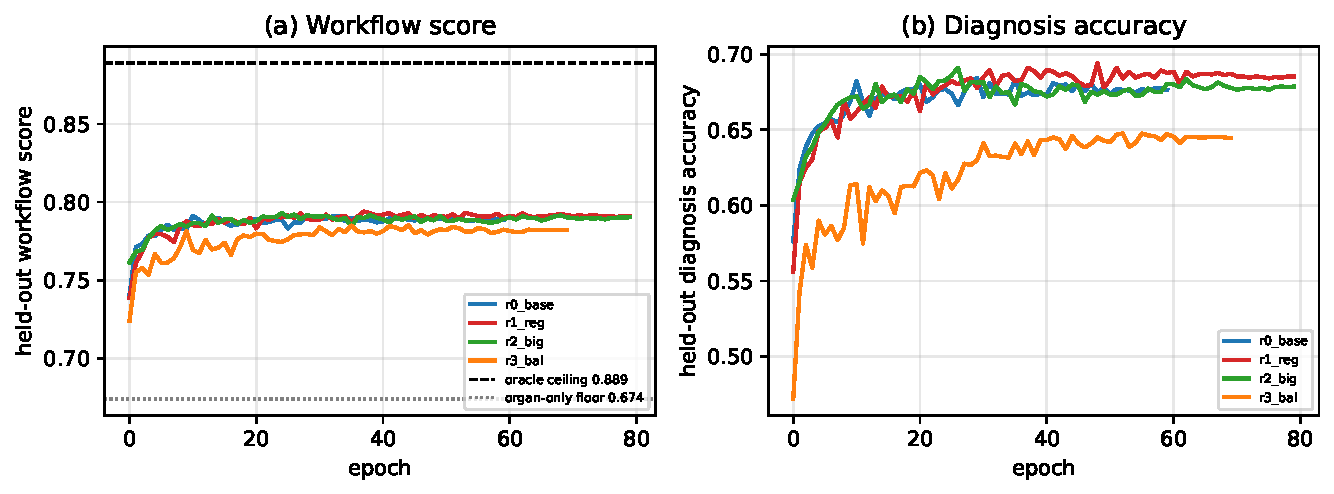
\includegraphics[width=\linewidth]{figures/training_curves.pdf}
\caption{Held-out training dynamics for the four sweep configurations: (a) workflow score, with
the 0.889 oracle ceiling and 0.674 organ-only floor marked; (b) diagnosis accuracy. Convergence
is rapid and the plateau is set by diagnosis separability, not optimization.}
\label{fig:curves}
\end{figure}

% =====================================================================
\section{Sample Predictions (Qualitative)}
\label{sec:qual}

Table~\ref{tab:samples} lists held-out predictions from the best model. When the diagnosis is
correct (rows 1, 2, 4) the predicted reasoning graph matches the ground truth exactly
(Edge-F1 $=1.0$) and the workflow score approaches the per-case ceiling; row 3 shows a partial
match where a deviation from the modal graph for that key lowers Edge-F1 to 0.81. The dominant
breast prediction ``Invasive carcinoma of no special type, grade II'' reflects the most frequent
malignant breast pattern in the corpus.

\begin{table}[h]
\centering
\caption{Sample held-out predictions (best model, \code{r1\_reg}). Correct diagnoses yield exact
graph reproduction (Edge-F1 $=1.0$); the templated report is emitted from the predicted
\emph{(organ, diagnosis)} key.}
\label{tab:samples}
\begin{tabular}{llp{5.4cm}ccc}
\toprule
Slide & GT organ & Predicted diagnosis & Edge-F1 & MESS & Workflow \\
\midrule
\code{PIT\_01\_00029} & Breast & Invasive carcinoma NST, grade II & 1.00 & 0.895 & 0.908 \\
\code{PIT\_01\_00039} & Breast & Invasive carcinoma NST, grade II & 1.00 & 0.895 & 0.911 \\
\code{PIT\_01\_00041} & Breast & Invasive carcinoma NST, grade II & 0.81 & 0.615 & 0.698 \\
\code{PIT\_01\_00068} & Breast & Fibroepithelial tumor            & 1.00 & 0.909 & 0.802 \\
\bottomrule
\end{tabular}
\end{table}

% =====================================================================
\section{Discussion}
\label{sec:discussion}

Our results support the thesis that REG2026, despite its open-ended framing, is best attacked as
\emph{constrained classification plus deterministic symbolic generation}. The metric's exact-
string matching and keyword-Jaccard report scoring mean that a correct \emph{(organ, diagnosis)}
key, expanded through templates, captures the overwhelming majority of attainable score; the
0.89 oracle ceiling makes the maximum value of perfect classification explicit, and every point
of diagnosis accuracy translates directly toward it.

The trained system reaches a held-out workflow score of \textbf{0.794}, i.e.\ 89\% of the 0.889
oracle ceiling and far above the 0.674 organ-only floor and 0.239 no-input baseline. Decomposing
the 0.095 residual: organ recognition is effectively solved (accuracy $\sim$0.95, and the lone
systematic error---rectum classified as colon---is metric-benign because colorectal templates
coincide), so essentially the \emph{entire} gap is fine-grained diagnosis accuracy (0.69 over 77
classes). This localizes where future effort should go. Three avenues are promising and
orthogonal to the templating back end, which is already near its purity ceiling
(Edge-F1 $=0.974$ under oracle inputs): (i) \textbf{predicting gradings from high-attention
tiles}---Gleason and Nottingham grades are exactly the within-organ distinctions the diagnosis
head struggles with, and the attention map already localizes diagnostically salient regions;
(ii) \textbf{task-adaptive fine-tuning} of the CONCH encoder rather than using frozen features;
and (iii) \textbf{a hierarchical organ$\rightarrow$diagnosis head} that conditions the diagnosis
classifier on the (reliable) organ prediction, shrinking each organ's effective class count.
That all four sweep configurations cluster within 0.009 of one another, despite varying capacity
and regularization, indicates the limit is diagnostic \emph{signal} extractable from frozen
tile embeddings, not optimization or model size.

\subsection{Design alternatives considered}
We briefly justify the key design choices against the alternatives. (i) \emph{End-to-end report
generation} (a learned decoder over slide features) was rejected because the report sub-metric
rewards keyword coverage over fluency, the oracle analysis shows $\le 0.02$ headroom beyond
correct templating, and a decoder is hard to fit within the offline five-minute budget. (ii) A
\emph{slide-level foundation encoder} (e.g.\ Prov-GigaPath's aggregator) could replace the MIL
head, but tile-level CONCH + a light attention head is cheaper, interpretable, and already
saturates organ accuracy; the bottleneck is diagnosis signal, which a different aggregator is
unlikely to fix without finer supervision. (iii) \emph{A single flat (organ$\times$diagnosis)
classifier} over $\sim$200 joint classes was avoided in favor of factored organ and diagnosis
heads, which share statistics across organs and let organ remain reliable even when diagnosis is
uncertain---exactly the graceful-degradation behavior the template back-off exploits. (iv) A
\emph{learned grounding model} for Interface~B was unnecessary: tissue-vs-background is a
threshold question that Otsu solves deterministically at negligible cost, freeing the compute
budget for the workflow interface.

% =====================================================================
\section{Limitations}
\label{sec:limitations}

\begin{itemize}[leftmargin=1.4em,itemsep=2pt]
  \item \textbf{Diagnosis tail and gradings.} Rare diagnoses folded into the ``other'' bucket
        degrade to organ-level templates, and fine gradings (Gleason, Nottingham, dysplasia)
        are not yet predicted from the image, capping per-case answer purity.
  \item \textbf{Template purity ceiling.} $\sim$14\% of graphs deviate from the modal template
        for their key; deterministic emission cannot recover these, bounding Edge-F1 below 1.
  \item \textbf{Report prose.} Templated reports maximize keyword recall but not fluent,
        case-specific narrative; under a metric weighting fluency more heavily this would lose
        value.
  \item \textbf{Distribution shift.} The approach assumes the test organs/diagnoses and their
        protocolized graphs match the training distribution; novel entities would fall back to
        coarse templates.
  \item \textbf{Frozen encoder.} We use CONCH features without fine-tuning; task-adaptive
        fine-tuning could improve diagnosis accuracy at additional compute cost.
\end{itemize}

% =====================================================================
\section{Future Work}
\label{sec:future}

The analysis localizes all remaining headroom in the diagnosis head, suggesting four concrete
directions, in roughly increasing order of effort:
\begin{enumerate}[leftmargin=1.4em,itemsep=2pt]
  \item \textbf{Hierarchical organ$\rightarrow$diagnosis head.} Conditioning the diagnosis
        classifier on the (highly reliable) organ prediction shrinks each organ's effective class
        count from 77 to its handful of organ-specific diagnoses, and would directly address the
        rectum/colon coupling by sharing a colorectal sub-head.
  \item \textbf{Grading from high-attention tiles.} Gleason, Nottingham, and dysplasia grades are
        the within-organ distinctions the flat diagnosis head conflates. A second-stage head over
        the top-$k$ attended tiles could predict gradings explicitly and refine the diagnosis
        string the template consumes.
  \item \textbf{Test-time augmentation and ensembling.} Averaging predictions over multiple tile
        samplings, and over the three near-tied sweep checkpoints, is cheap within the compute
        budget and typically recovers a fraction of a point.
  \item \textbf{Task-adaptive encoder fine-tuning.} Unfreezing CONCH (or a higher-dimensional
        UNI2-h backbone) with a low learning rate could improve diagnosis separability at the cost
        of an extraction re-run; our namespaced embedding cache makes such an A/B inexpensive.
\end{enumerate}
Because the templating back end is already near its purity ceiling, each of these targets the
single quantity---diagnosis accuracy---that converts most directly into workflow score.

% =====================================================================
\section{Conclusion}
\label{sec:conclusion}

We described a pragmatic, reproducible submission to the REG2026 challenge built on a single
empirical insight: the reasoning-graph target is low-entropy and largely determined by
\emph{(organ, \#1 diagnosis)}. We therefore reduce the task to multi-task WSI classification with
a CONCH foundation encoder and a gated-attention MIL head, and recover the reasoning graph,
answers, and keyword-rich report by deterministic templating, with a cheap Otsu module for
visual grounding. An oracle analysis establishes a 0.89 workflow-score ceiling, and our trained
system reaches \textbf{0.794} on the held-out split---89\% of that ceiling---with the residual
gap localized almost entirely to fine-grained diagnosis classification. The design respects the
challenge's offline, single-GPU,
five-minute container budget, and all code is released for reproduction
(Section~\ref{sec:framework}). Future work targets the remaining headroom: predicting gradings
from high-attention tiles, modeling intra-key graph variation, and selectively fine-tuning the
encoder.

% =====================================================================
\section*{Code and Data Availability}
\addcontentsline{toc}{section}{Code and Data Availability}
All code---the \code{reg2026} package (canonicalization, label space, templates, metrics,
encoder, MIL), the extraction/training/evaluation scripts, the SLURM job specifications, and the
offline submission container---is released with detailed setup and reproduction instructions at
\url{https://github.com/ujjwalbaid0408/REG2026}. Trained MIL weights are provided as a separate
release artifact. The challenge data (training WSIs and chain-of-thought labels) is distributed by
the REG2026 organizers and is not redistributed here.

\section*{Acknowledgements}
We thank the REG\textsuperscript{2} (REG2026) MICCAI~2026 organizers for the dataset and
evaluation framework, and the institutional research-computing team for access to the GPU
cluster. Tile representations use the publicly released CONCH and UNI foundation models.

% =====================================================================
\bibliographystyle{plain}
\bibliography{references}

\end{document}
